\documentclass{jarticle}
\usepackage{rsj}
\usepackage[dvipdfmx]{graphicx}
\graphicspath{{figs/}}
\usepackage{url}

\begin{document}

\title{RSJレポートのテンプレート}
\author{◯源 頼朝 (東京大学)}

% 行間の設定
\setlength{\baselineskip}{4.4mm}
\maketitle
\thispagestyle{empty}
\pagestyle{empty}

\section{はじめに}

本稿はRSJレポートのテンプレートである~\cite{Sakai}.

本稿における「、」や「。」は、\verb|make pub|を実行することで、「,」や「.」に変更される。

図は\figref{nowprinting}や\tabref{sample}として参照する.

\begin{figure}[tbh]
 \begin{center}
  \begin{minipage}{0.3\columnwidth}
   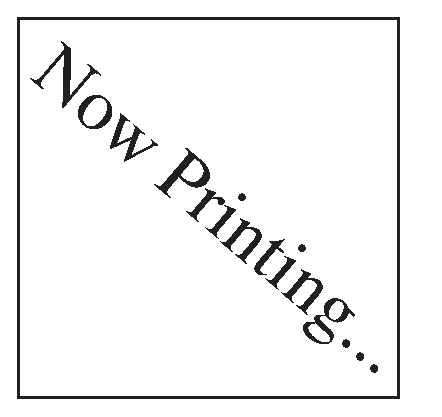
\includegraphics[width=\columnwidth]{nowprinting.eps}
   \caption{eps図の参考例}
  \end{minipage}
  \hspace{0.15\columnwidth}
  \begin{minipage}{0.3\columnwidth}
   
\includegraphics[width=\columnwidth]{dj.jpg}
   \caption{jpg図の参考例}
  \end{minipage}
  \label{figure:nowprinting}
 \end{center}
\end{figure}

\begin{table}[tbh]
 \begin{center}
  \begin{tabular}{|l|r|} \hline
  A1 & B1 \\
  A2 & B2 \\ \hline
  \end{tabular}
  \caption{図の参考例}
  \label{table:sample}
 \end{center}
\end{table}

\section{おわりに}

\small
\bibliographystyle{junsrt}
\bibliography{main}
\normalsize

\end{document}

